\newpage
\section{Discussion} \label{section:discussion}

\begin{comment}
the discussion, in which you connect the results to the research questions and the literature

aanpak log verwerking:
- totaliseren van de results
- actie research: wat ben ik aan het doen
- experimenteren in de praktijk
- deel uitmaken van het proces
- laten gebeuren
- valt me op dat .... -> content analyse
- cluster waarneming -> beschouwen: het valt me op dat .. en onderbouwing
- bottom up (logs) en top down (gesprekken)
- bij elk log -> wie wat waar; traceerbaar houden
=======
- iemand moet het nalezen op consistentie
- nalezen op vorm
- checken of de referenties nog kloppen

\end{comment}
The most common keywords within the observations in appendix ~\ref{appendixLoglines} are with the terms "Ampersand", "Api ","Concept", "Conceptual analysis",
"Interface", "Law", "Multiplicity", "Relation" and "Rule".
These are terms that in most cases are part of the Ampersand method.
Only the term "law" refers to the case itself.

This chapter focuses on the relationship between the results (see section~\ref{Results} and the sub-questions.
A separate section has been included for each sub-question in which the sub-question is answered on the basis of the included results.
Each paragraph contains a reference to the respective results to which it relates, in whole or in part.

Many observations were made during the research.
The analysis showed that not all observations are relevant.
These were therefore not included in the further analysis.
Even observations that were initially assigned to a category turn out to be irrelevant on closer inspection and have been included as such.

\subsection{Ampersand knowledge}\label{subsection:ampersand-knowledge}

When working with Ampersand, a development environment must first be set up. 
Ampersand's documentation assumes that XAMPP~\footnote{\url{https://github.com/AmpersandTarski/documentation/blob/master/installing-ampersand/installing-the-tools-manually.md}} can be configured for this become.
The preferred configuration is done with the help of Docker.
If there is little or no knowledge of Docker, you can choose to set up XAMPP.
However, it was not possible to get the local installation working with the help of the documentation.
However, with help we managed to get it working in the Docker environment.
So starting with Ampersand, it's not just Ampersand that needs to be studied, it's also the environment in which it operates that needs to be studied.
This part always works.
Setting up the environment and Ampersand is also fine from the website and from Github.
There is also some information on Stackoverflow.
But beyond that there is nothing to be found outside of a number of scientific articles.
Fortunately, there are articles like \cite{de_swart_ampersand_2011} that explain Ampersand.

The sub-question "\acrlong{RQ1}" examines the knowledge of the software engineer when using Ampersand.
To answer this question we can use the next results: \sref{sbbs:useful-1}, \sref{sbbs:useful-2}, \sref{sbbs:useful-3}, \sref{sbbs:useful-4}, \sref{sbbs:ampersand as method-1}, \sref{sbbs:ampersand as method-2}, \sref{sbbs:ampersand as method-3}, \sref{sbbs:ampersand as method-4}, \sref{sbbs:design-2}, \sref{sbbs:ampersand as tool-1}, \sref{sbbs:ampersand as tool-2}, \sref{sbbs:ampersand as tool-3} and \sref{sbbs:ampersand as tool-4}


In order to be able to use Ampersand itself, in addition to knowledge about the structure of the environment, knowledge of Ampersand itself is required.
There is not a lot of information about Ampersand on the internet and there are examples, but they do not cover the whole load.
As with any tool and method, knowledge will have to be kept up to date to keep Ampersand usable.
This is not specific to Ampersand, but of course also applies to Ampersand.
(Ref. to \sref{sbbs:useful-1})


Proper use of Ampersand requires proper documentation setup.
This setup consists of knowledge of the way Ampersand handles the information in the scripts.
The positioning of the meaning of the Terms and the Relationships and the purpose of the Rule and the use of includes.
One should be aware that the meaning, purpose and definitions appear directly in the documentation and the inclusions help determine the order of the story and that this should be a unifying story.
Agreement must be reached in advance about the structure of the spelling, the reference to legislation and regulations.
The notation method, the naming convention of Concepts and Relations must also be unambiguous in order to have a consistent and professional appearance.
As one of the interviewees pointed out, when analysis and documentation needs to be done, why not through Ampersand.
Unfortunately, the researcher started to standardize somewhat later, so that this was not implemented everywhere.
(Ref. to \sref{sbbs:useful-1}, \sref{sbbs:useful-2})


When working with Ampersand and going through the text, it seems logical to go through the text chronologically.
However, this will not always work and a method must be found to maintain the overview.
Maintaining overview is difficult when using Ampersand because the source can be huge.
This aspect has been approached in various ways.
The source text in XML has been looked at, with the intention of adding extra XML tags.
The intended side effect of this was that we could generate the model from the XML.
This didn't work because the original XML is way too complex and would make the XML parsing very complex as well and the work has to be redone with a new version of the law.
The RTF format was like a Word document and could be provided with comments.
The same was true for the PDF format.
\F{Annotation}{An annotation tool is required to maintain an overview of the text to be processed. 
This prevents things from being processed twice or not.} is also possible here and one can also underline with colors.
In the end, the old-fashioned choice was made for the combination of hard copy and the PDF.
Hard copy for streaking and writing and the PDF for searching and copying text.
(Ref. to \sref{sbbs:useful-3})



Maintaining the overview in the created scripts is also a challenge.
By using Visual Studio\footnote{\acrlong{vsc} observations are not categorised, no direct involvement with Ampersand}  there are no \F{refactor}{There is a need to enable refactoring within an IDE.
We can then prevent issues when removing, for example, Includes.
Changing naming or viewing where a Concept or Relation occurs is highly desirable.} options.
Visual Studio also seems to lack integration between the scripts.
The consequence of this is that it is possible that the same Concepts and also Relationships are defined in several places.
By not being aware of the overlap, a different definition can occur for the same Concept.
The differences will not be very large, but certainly worded differently.
This only came to light when the documentation was generated.
The advantage of working with text and generating the model from it appears to be a disadvantage here.
(Ref. to \sref{sbbs:ampersand as method-4}, \sref{sbbs:ampersand as tool-2})

When creating a script where the analyst does not yet have that much experience, it happens that the meaning and purpose are not filled in.
This is caused by the analyst being too busy getting Relations and Rules working within the scripts.
The consequence of this is that meanings and purposes are not filled in and they therefore become visible in the \acrshort{ca}.
It is almost impossible to update it afterwards.
This can be prevented by working as a team, where the team members keep each other sharp on these matters and there is experience in the team.
(Ref. to \sref{sbbs:useful-4})


\begin{comment}
@startuml
skinparam handwritten true
node "Generiek" {
  [Persoon]
  [Inschrijving]
  [etc]
}
node "Arts" {
  [Component Arts]
}
node "Tandarts" {
  [Component Tandarts]
}
node "etc" {
  [Component etc..]
}
[Persoon] --> [Component Arts]
[Inschrijving] --> [Component Arts]
[Persoon] --> [Component Tandarts]
[Inschrijving] --> [Component Tandarts]
[Persoon] --> [Component etc..]
[Inschrijving] --> [Component etc..]
@enduml
\end{comment}
Article 3(1) of the \acrshort{big} states that there are several registers.
In order to implement this, an attempt has been made to install a single register in combination with the shared piece.
The \F{shared components}{Dealing with shared components such as Concepts, Relations or Patterns. This both within a project and across the projects.} appear in each register and include the person registration and the registration leading to the actual registration.
The implementation of the prototype of a profession with the common part was no problem (\ref{fig:arts-deploy}.
Until the next profession was established (\ref{fig:tandarts-deploy}).
 \begin{figure}[h]
     \centering
     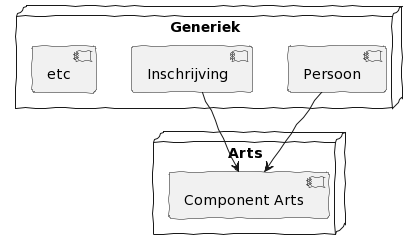
\includegraphics[width=0.4\textwidth]
        {arts.png}
     \caption{Arts with generiek}
     \label{fig:arts-deploy}
 \end{figure}
 \hfill
 \begin{figure}[h]
     \centering
     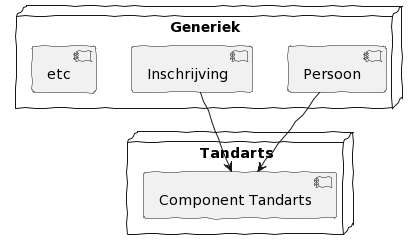
\includegraphics[width=0.4\textwidth]
        {tandarts.png}
    \caption{Tandarts with generiek}
    \label{fig:tandarts-deploy}
 \end{figure}
\\
Then the first professional group was removed from the database and the common data was also removed and the second group was fully initiated.
The method of building specific professional registers in this way is not (yet) supported by Ampersand, so it has to deployed all in once (\ref{fig:monoliet-deployment}).
\begin{figure}[H]
    \centering
        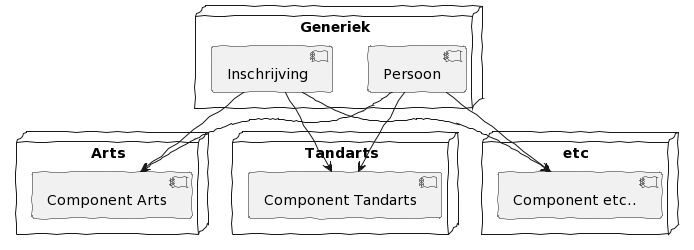
\includegraphics[width=1\textwidth]
            {monoliet.png}
        \caption{Deployment in once}
    \label{fig:monoliet-deployment}
\end{figure}
If this does not work for this law, it will also not work for links with other registers where data and the associated management software must be shared.
(Ref. to \sref{sbbs:ampersand as tool-2})



Every organization has an authorization mechanism for the software.
The \acrshort{cibg} uses a JWT mechanism.
In the research I encountered an authorization mechanism when creating the Rules and when building the Interface.
I have not found out whether it is possible to integrate this with the organization's own authorization mechanism.
(Ref. to \sref{sbbs:ampersand as tool-3})


To be able to use Ampersand correctly, knowledge of relation algebra is required.
You use this algebra as a Software engineer to build rules and relationships.
The knowledge of multiplicity is indispensable when creating rules and relationships.
The naming convention is partly present within Ampersand.
Some elements, such as pattern, for example, are capitalized.
Concepts always start with a capital letter.
For example, there are a number of fixed agreements.
There are no agreements regarding the use of, for example, relation names.
For matters for which Ampersand has no constraint, a set of best practices could be set up.
(Ref. to \sref{sbbs:ampersand as method-1}, \sref{sbbs:ampersand as method-2}, \sref{sbbs:ampersand as method-3})


The Software engineer needs limited knowledge of Latex and HTML to influence the \acrshort{ca}.
In many cases this is not necessary because Ampersand handles this excellently.
However, there are opportunities to intervene and provide direction here.
(Ref. to \sref{sbbs:design-2})


The Software engineer must know how to control Ampersand in terms of the use of includes.
These includes control the \acrshort{ca}, but are also used when building the application.
If the includes are not specified where they are needed, the build will fail and when it is specified where not necessary, the build goes well and the \acrshort{se} has the option to send the \acrshort{ca} on content.
The development of extra functions that have not yet been included within Ampersand is done using PHP.
The Software engineer therefore needs knowledge of PHP to develop these functions and of course Ampersand to be able to actually deploy these functions.
(Ref. to \sref{sbbs:ampersand as tool-1},  \sref{sbbs:ampersand as tool-4})


The team that Ampersand maintains and wants to expand is very active.
The involvement is also apparent from the rapid resolution of issues that occurred.
(Ref. to \sref{sbbs:useful-1})

\subsection{Ampersand core in wet BIG}\label{subsection:ampersand-core-in-wet-big}
With sub-question "\acrlong{RQ2}" we want to know what is in the \acrlong{ca}.
For this appendix~\ref{appendixContentAnalysis} is included.
The \acrlong{ca} contains the Concepts, Relations and Rules (see figure~\ref{fig:LogicalDataModel}).
\begin{figure}[!htp]
    \centering
        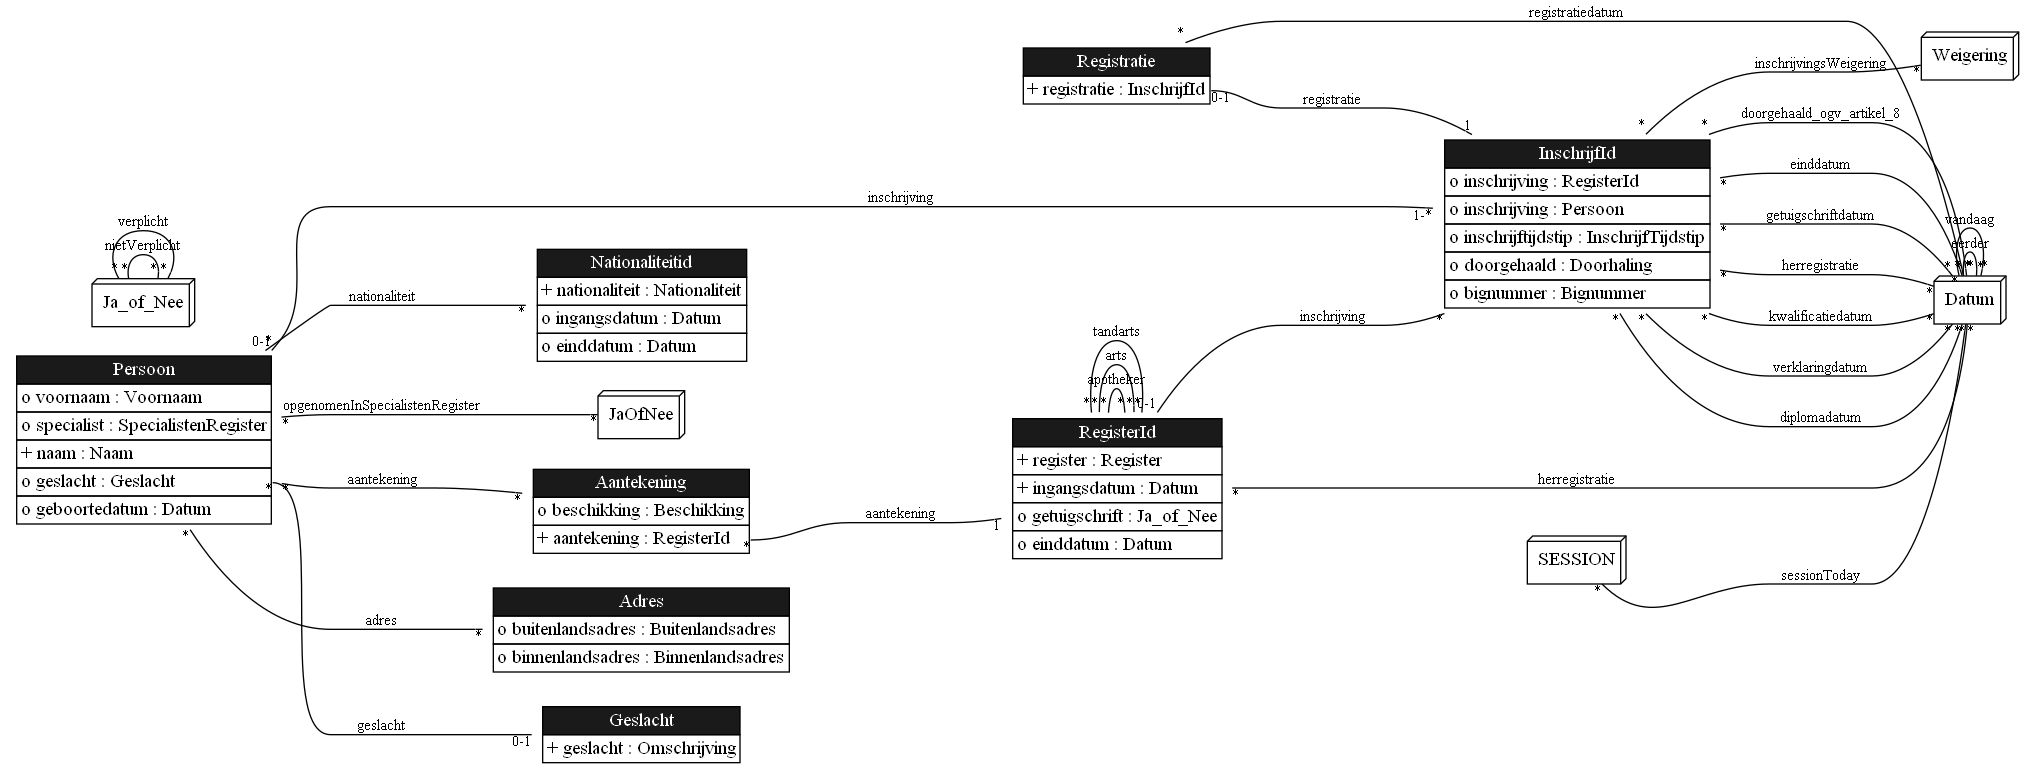
\includegraphics[width=1\textwidth]
            {../images/LogicalDataModel.png}
        \caption{LogicalDataModel from the \acrlong{ca}}
    \label{fig:LogicalDataModel}
\end{figure}
The \acrlong{ca} is not completed because not all articles and related regulations has been analyzed.


\subsection{Setup law for Ampersand}\label{subsection:setup-law-for-ampersand}
Reading and understanding the legal texts requires special skills.
For example, article 13 paragraph 1, here it reads:
\textit{"Indien bij besluit van Onze Minister inschrijving in een register is geweigerd, de afgifte van een verklaring van vakbekwaamheid wordt geweigerd of een beroepsbeoefenaar de bevoegdheid zijn beroep uit te oefenen heeft verloren omdat hij de aanvraag tot inschrijving of tot afgifte van een verklaring gebaseerd heeft op valse kwalificaties, kan Onze Minister besluiten, onverminderd de hoofdstuk V van de Algemene verordening gegevensbescherming, de bevoegde autoriteiten van andere staten dan de staten bedoeld in artikel 31a, eerste lid, van de Algemene wet erkenning EU-beroepskwalificaties, daarvan in kennis stellen."}
Due to the length of the sentences and the many parentheses, the analysis of a piece of legal text can only be read properly by a person with experience in reading legal documents.

The sub-question "\acrlong{RQ3}" deals with the law, in the case of the \acrshort{big}, and the way in which it can be analyzed and processed using Ampersand.
To answer this question we can use the next results: \sref{sbbs:useful-5}, \sref{sbbs:design-3}, \sref{sbbs:design-4}, \sref{sbbs:analysing law-1}, \sref{sbbs:analysing law-2}, \sref{sbbs:analysing law-3}, \sref{sbbs:analysing law-4}, \sref{sbbs:analysing law-5}, \sref{sbbs:design-6}


Interviews paint a picture of a law that originated in the 19th century.
Although this has been adapted to the current times, the structure is not equipped for a one-to-one translation to an information system.
It has been indicated that there are new laws that are much better suited for translation, such as, for example, "Regeling bewijsstukken sociale hygiëne Drank- en Horecawet 2015".
Since we have not analyzed any other laws, it cannot be determined whether this is the case.
But the \acrshort{big} is a large and complex law, according to a lawyer at the \acrshort{cibg}.
(Ref. to \sref{sbbs:analysing law-5})


Analyzing the law requires legal knowledge.
Reading the legal texts also requires the necessary experience.
Analyzing the law is usually not the domain of a business analyst.
At the start of the analysis, a team should be set up that should include at least an analyst and a lawyer.
The analyst for building and managing the script and the lawyer for the translation of the law into Concepts and Relationships.
This ensures consistency and completeness of the analysis.
It has been found that even a lawyer can understand the concepts and the relationships of conceptual analysis.
As a result, the cooperation on this point will run smoothly.
(Ref. to \sref{sbbs:analysing law-2}) 


By starting with the analysis of the law with the help of a lawyer, an overview can be obtained at an early stage of the content and structure of the law.
By looking at the structure, the analyst can better understand what the law is about.
The structure can also help to determine the structure of the patterns.
It's certainly not the case that every chapter is a separate pattern, but it certainly influences the setup of the \acrlong{ca} and thereby help to gain an overview of the law and, on the other hand, of the analysis to be performed.
(Ref. to \sref{sbbs:analysing law-4}, \sref{sbbs:analysing law-3})


In order to extract the correct data and understandable data from the source text, experience is required in reading and interpreting the legal texts.
Some laws lend themselves to this better than others.
In addition to the understandable law, a law analyst is also needed.
(Ref. to \sref{sbbs:useful-5}, \sref{sbbs:useful-6})


The set-up of the \acrshort{big} is limited in nature.
The limitation is that it does not include lifecycle management.
The law deals with how a person can register and deregister.
The law also specifies the requirements that the person must meet in order to remain registered.
This per is partly general and partly per register.
The missing lifecycle management relates to the management of the registers themselves.
The law states that they are there, in decrees more are added.
But nowhere is it written what should be done when cleaning one or more registers.
(Ref. to \sref{sbbs:design-3},  \sref{sbbs:design-4})


In the initial analysis of an Ampersand assignment, the scope will be determined.
This scope is often more than the law itself.
In the case of \acrshort{big} there is a list of rules and decisions (see~\ref{list:ass-laws-regulations}.
In addition to the immediately findable legislation and regulations, there are also overarching regulations that play a role.
In some cases it is legislation and regulations that influence the scope, but it is rules that are determined by another source.
Think of the NORA architecture rule, the formatting rules of addresses by BRP.
So a set of people are needed to determine the scope.
(Ref. to \sref{sbbs:analysing law-1}, \sref{sbbs:design-6})

\subsection{Ampersand for government organization}\label{subsection:ampersand-for-government-organization}
The sub-question "\acrlong{RQ4}" focuses on the use of Ampersand within the \acrshort{cibg} organization.
The information systems that are not based on legislation and regulations and which aim to monitor data quality are often the registers.
\acrshort{cibg} builds, manages and monitors this data through registration systems.


In conversations with an architect of the \acrshort{cibg}, maintenance of the Ampersand model is discussed.
When a model is set up, this results in a certain version of the model.
The model consists of a database model and the other software and an \acrshort{ca}.
This model can be implemented by a development team.
Legislation will certainly be amended during the software's life cycle.
By including these changes in the model, a new model is created.
Ampersand does not provide any resources to guide the conversion from the old model to the new model.
The development team will therefore have to make an analysis of the old and the new situation and have to develop conversion software for that.
This is a method that is different from usual.
Usually when changing the software, the changes in the database are taken into account immediately.
The advantage of a new model is that the software does not have to do with legacy.
It is therefore always a state-of-the-art model.
The downside is that the conversion is likely to be complex.
Data that was previously valid may be invalid in a subsequent model.
(Ref. to \sref{sbbs:useful-9}, \sref{sbbs:design-8})


Ampersand is declarative and reactive, so the Ampersand implementation always responds to the current situation through validations.
The execution of management processes is left to the \acrshort{rk}, which supports the process handling.
(Ref. to \sref{sbbs:registry systems-1})


Although Ampersand is intended as a design and prototyping tool, it does have APIs at its disposal.
This can only be obtained from log lines and apparently not intended as a means of communication from external systems.
This is also apparent from the fact that no API description is made in, for example, Swagger~\footnote{\url{https://swagger.io}}.
But it can work that way.
It is possible to communicate with the Ampersand core from an external source.
The return actions from the called APIs are not provided with a code but text.
As proof of concept, calls were made from Postman~(see figure~\ref{fig:postman-get-person}) to Ampersand and that worked as expected, see figure~\ref{list:postman-output}.
(Ref. to \sref{sbbs:useful-8})
\begin{figure}[ht]
    \centering
    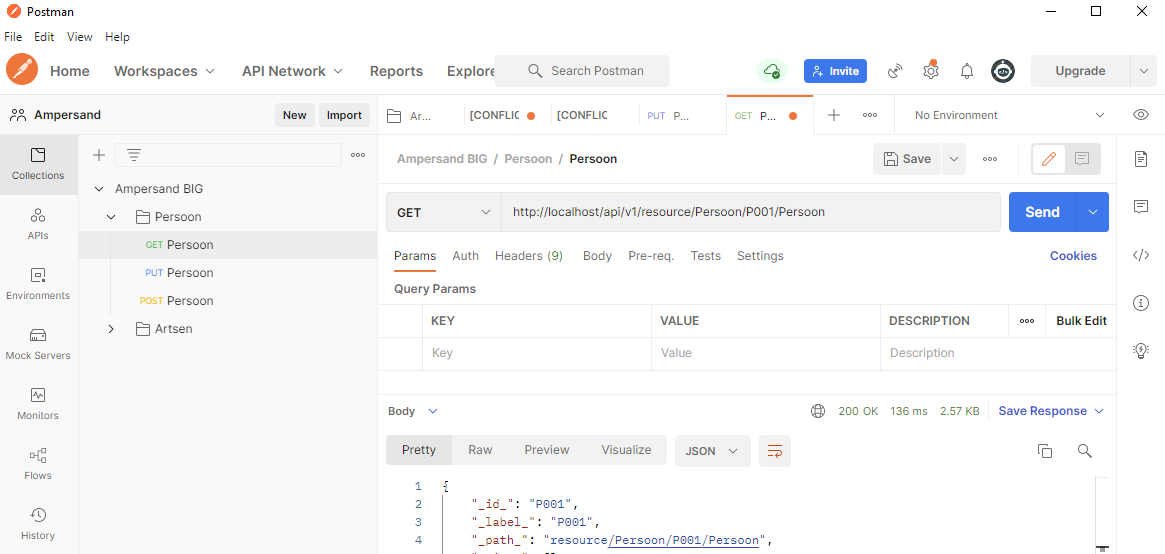
\includegraphics[width=\textwidth]{/postman_GET.PNG}
    \caption{Postman GET Person}
    \label{fig:postman-get-person}
\end{figure}

\begin{lstlisting}[language=json,firstnumber=1,caption={Postman output from GET Person},captionpos=b,label={list:postman-output}]
{
    "_id_": "P001",
    "_label_": "P001",
    "_path_": "resource/Persoon/P001/Persoon",
    "_view_": [],
    "Persoon": {
        "_id_": "P001",
        "_label_": "P001",
        "_path_": "resource/Persoon/P001/Persoon/Persoon",
        "_view_": [],
        "_ifcs_": []
    },
    "Naam": "Edelaar",
    "Voorna_40_a_41_m_40_en_41_": "Gerard",
    "Geslacht": {
        "_id_": "M",
        "_label_": "M",
        "_path_": "resource/Persoon/P001/Persoon/Geslacht/M",
        "_view_": [],
        "Code": {
            "_id_": "M",
            "_label_": "M",
            "_path_": "resource/Persoon/P001/Persoon/Geslacht/M/Code",
            "_view_": [],
            "_ifcs_": []
        },
        "Omschrijving": {
            "_id_": "Man",
            "_label_": "Man",
            "_path_": "resource/Persoon/P001/Persoon/Geslacht/M/Omschrijving/Man",
            "_view_": [],
            "_ifcs_": []
        },
        "_ifcs_": []
    },
    "Adres": [
        {
            "_id_": "adres1",
            "_label_": "adres1",
            "_path_": "resource/Persoon/P001/Persoon/Adres/adres1",
            "_view_": [],
            "_ifcs_": [
                {
                    "id": "Adres",
                    "label": "Adres"
                }
            ]
        }
    ],
    "Geboortedatum": "2000-01-01",
    "Nationaliteit": [
        {
            "_id_": "0001",
            "_label_": "Nederlandse",
            "_path_": "resource/Persoon/P001/Persoon/Nationaliteit/0001",
            "_view_": {
                "nationaliteit": "Nederlandse"
            },
            "_ifcs_": []
        }
    ],
    "Inschrijving": [
        {
            "_id_": "I001",
            "_label_": "I001",
            "_path_": "resource/Persoon/P001/Persoon/Inschrijving/I001",
            "_view_": [],
            "_EMPTY_": {
                "_id_": "I001",
                "_label_": "I001",
                "_path_": "resource/Persoon/P001/Persoon/Inschrijving/I001/_EMPTY_",
                "_view_": [],
                "_ifcs_": [
                    {
                        "id": "Inschrijving",
                        "label": "Inschrijving"
                    }
                ]
            },
            "_ifcs_": []
        }
    ],
    "_ifcs_": []
}
\end{lstlisting}


By using Ampersand as a design tool, a prototype is available at an early stage.
This prototype can be converted into a website with the appearance of a \acrshort{cibg} website by means of HTML additions and CSS adjustments.
Test cases can already be developed at an early stage on the basis of this prototype and the functions of the prototype, by using the APIs, can be used as a stub in the development of the system.
(Ref. to \sref{sbbs:ampersand as method-6})


An organized ICT organization such as the \acrshort{cibg} has an architecture that new software must comply with.
One of the developments in the \acrshort{cibg} is the set-up of the \acrshort{rk} (see interview developer Appendix~\ref{par:interview-developer}).
\acrlong{rk} its terminology includes "zaken" and "producten".
Every service, read implementation of a law, we call a product.
There are default items that always appear in every registry.
These are pre-modeled in \acrshort{rk}.
This includes a foundation for each registry and can be expanded to meet the needs of the registry.
The basis is the minimum common denominator of the registers.
Extendable to specific elements arising from the law.
There is certainly overlap in the data obtained from the analysis of the great law and the \acrshort{rk}.
About 80\% of the \acrshort{rk} is generic and the other 20\% is custom.
All new registers therefore have the same basic principles and largely run on the same software.
However, a mapping still has to take place from the found Concepts from the law to \acrshort{rk}.
The overlap in this is not always immediately visible.
Within the \acrshort{rk} the term product is used, within the \acrshort{big} this product is a register or possibly even all registers.
The latter depends on the implementation.
This mapping must be made explicit and has not been taken into account in this study.
The developer has indicated that full integration of the Ampersand model is not possible, due to the aforementioned overlap of the Concepts.
However, the modified part of the \acrshort{rk} can be used for the Ampersand model implementation.
Calculations are not standard in Ampersand, but this can be solved by writing external functions or even solving it in \acrshort{rk}.
(Ref. to \sref{sbbs:registry systems-2}, \sref{sbbs:useful-7}, \sref{sbbs:design-1})

In RAP there is a tool called Atlas, it shows the context and the patterns.
In addition, all Concepts, Rules, Properties and Relations, with hyperlinks to the components.
Via the hyperlink details of the item inclusion a relationship diagram is shown.
Very nicely executed and very useful when working in RAP.
This tool is a viewer on the information and it is not possible to also edit the \F{information in Atlas}{Being able to edit the Atlas information from Atlas}.
However, the case study was so large that the RAP environment was not sufficient.
RAP does not support Includes and has been used extensively.
Unfortunately, \F{Atlas availability}{Make Atlas available outside the RAP environment.} cannot be implemented outside of RAP.
(Ref. to \sref{sbbs:ampersand as tool-5})


As a novice user of Ampersand it takes a while to master Relation algebra.
That is why an excel sheet has been made to make the Relations visible with the associated multiplicity.
This is a method that is easy to use initially.
The disadvantage of this approach is the consistent transfer of Concepts and Relations.
We need to double track this information and redundancy in the field of data will certainly go wrong.
When Concepts disappear, they must also be removed from Excel or Relations that do change due to new insights must be adjusted here.
In short, this does work for small, well-arranged projects, but for larger ones, gaps will quickly arise and this no longer represents reality.
The result was that the excel sheet was used a lot in the beginning and not anymore later on.
(Ref. to \sref{sbbs:ampersand as method-2})


To be able to perform the analysis properly, it is not enough to have one person perform it, as in the study.
Due to inexperience with the use of Ampersand, the initial appointment set was not created.
Ampersand's knowledge is only really gained during the execution.
In addition, the amount of legal texts is so large that it cannot be passed through within a reasonable period of time.
In addition to IT knowledge, legal knowledge is also required, on the one hand to be able to read the law and on the other hand to find the implicitly related laws and regulations.
Depending on the size of the legislation and regulations to be analyzed and the lead time that one wants to use, a team size will be determined.
A team consists of at least a lawyer and an (Ampersand) experienced business analyst.
A third person to validate the data.
(Ref. to \sref{sbbs:ampersand as method-5})


Ampersand is a completely new method for the \acrshort{cibg} organization.
People have never heard of it and unfortunately there is not much to be found about it.
This means that people are not positive about it in advance, calling NIH~\footnote{not invented here}\citep{antons_assessing_2017}.
It is expected that the Ampersand method will take more time than the current method (see interview~\ref{int:I-1.8}) and is wary of anything new.
It is clear that the advantages of the method are not yet understood.
Benefits such as working directly on the source, generating a prototype from there (see appendix~\ref{appendixPrototype}) with all validations and full conceptual specifications (see appendix~\ref{ConceptualAnalysis}).
Having a prototype makes it possible to build test scenarios at an early stage and with the \acrlong{ca} you can start building immediately.
(Ref. to \sref{sbbs:design-5}, \sref{sbbs:ampersand as method-6}, \sref{sbbs:useful-11})


Although Ampersand is new to the \acrshort{cibg} organization, one of the interviewees pointed out (see interview analist~\ref{par:interview-analist}) that documentation in the form of a design should be made with each new register.
According to the analyst, it should not matter which tool is used for this.
The advantage of Ampersand is that it generates a model from the analysis instead of the usual model-to-text approach.
A model is made of each pattern.
See for example the Pattern for \mbox{Person} (see script~\ref{lst:persoon}).
This results in the model of figure~\ref{fig:pattern-persoon}.
(Ref. to \sref{sbbs:useful-10}, \sref{sbbs:ampersand as method-7}, \sref{sbbs:design-7})
\begin{figure}[H]
    \centering
        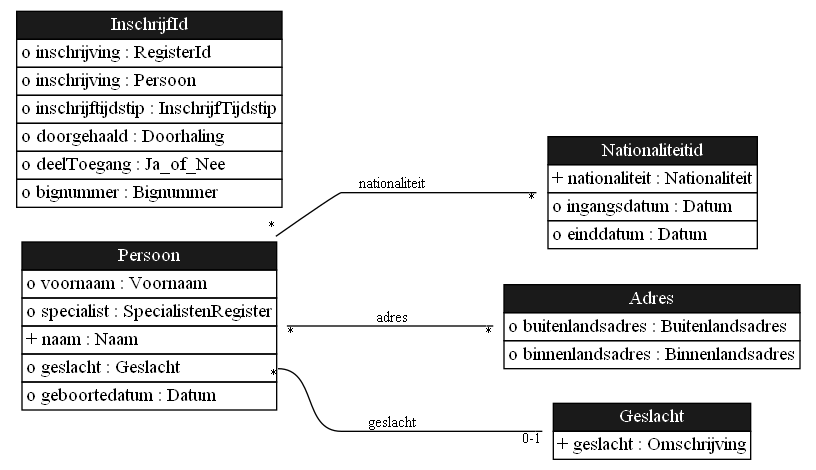
\includegraphics[width=1\textwidth]
            {../images/CDPatternPersoon.png}
        \caption{Pattern Persoon}
    \label{fig:pattern-persoon}
\end{figure}


The design of registry systems has no specific points of attention.
Part of the research question was about designing for registry systems.
Other than the source specific link, the \acrshort{big}, no specifics were found for registry systems.
The translation of this law into an information system results in a register.
The requirements of the register are laid down in law.
This concerned, among other things, the identifying data of a registration.
In article 3, paragraph 1~\footnote{\url{https://wetten.overheid.nl/jci1.3:c:BWBR0006251&hoofdstuk=II&paragraaf=1&article=3&z=2022-04-01&g=2022-04-01}} it says it's about registers.
This also explains why there are not much observations regarding registry systems.
The register system is therefore not an isolated one, but a consequence of the fact that the source is a law.

\subsection{Limitions}\label{sbs:limitions}
The focus of the research was on executing the process to construct at a \acrshort{ca} and a prototype.
The time for this is in principle 2 quarters.
We have moved a little over time and it turns out that it is not possible to fully analyze just a law like \acrshort{big}.
The limitation we encountered is that there is a shortage of time.
This has to do with an optimistic estimate of what work can be done.
The start with Ampersand is more difficult than it seems.
The \acrshort{big} is much larger and more complex than it first appears.
Reading the law is also an art.
The law has many references to other laws.
This resulted in an \acrshort{ca} which is not complete.
The process did provide enough material to make several statements (see section~\ref{conclusions})

\begin{comment}
discussie voer

niet alle observaties zijn gebruikt

Een risico dat gelopen wordt door de moeilijke teksten is dat er niet zorgvuldig genoeg gelezen wordt en er eigen interpretatie plaatsvindt.
Dat risico neemt toe, naar mate het domein vertrouwder is voor de onderzoeker. 
Dus de keerzijde van de \acrshort{ar} aanpak is een bias op de inhoud.

De overall aanpak van de analyse van de wet is om eerst een overzicht te krijgen van de wet.
Het doorlopen van de wet en de highlights van de artikelen helder te krijgen.
Dit sluit aan bij het idee om de indeling op voorhand te maken


Vanuit verschillende interviews werd het statement gemaakt of \acrshort{big} wel de meest geschikte wet is om deze met Ampersand te analyseren.
Reden is dat de wet van orgine heel oud is~\ref{section:big}. 
De wet is verschillende malen bijgewerkt, maar de structuur is niet simpel om te zetten naar een ICT-systeem.
Daarnaast bevat de wet zeer veel impliciete en expliciete verwijzingen naar andere wet- en regelgeving.
En de wet is zelf niet expliciet genoeg.
Er zijn behoorlijk veel interpretatie mogelijkheden.
-> leidt tot sneller aansluiten bij de tot stand koming van de wet
-> vroegtijdige analyse van de haalbaarheid
-> alternatieve aanpak etc.
\end{comment}

